\documentclass[acmtog]{acmart}
% Title portion
\title{Assignment 3 : Cloth Simulation using Mass-Spring System} 
\author{Name:\quad Tianyuan Wu  \\ student number:\quad 63305667
	\\email:\quad wuty@shanghaitech.edu.cn}

% Document starts
\begin{document}
\maketitle

\vspace*{2 ex}


\section{Introduction}
In this assignment, I implement a simple cloth animation using a mass-spring system.
The implementation is in C++11 with OpenGL. This implementation contains 3 parts:\\
(1) Triangle mesh builder / Cloth Renderer\\
(2) Mass spring system solver\\
(3) Constraint systems\\
A demo of my implementation is shown below:
\begin{figure}[H]
	\centering
	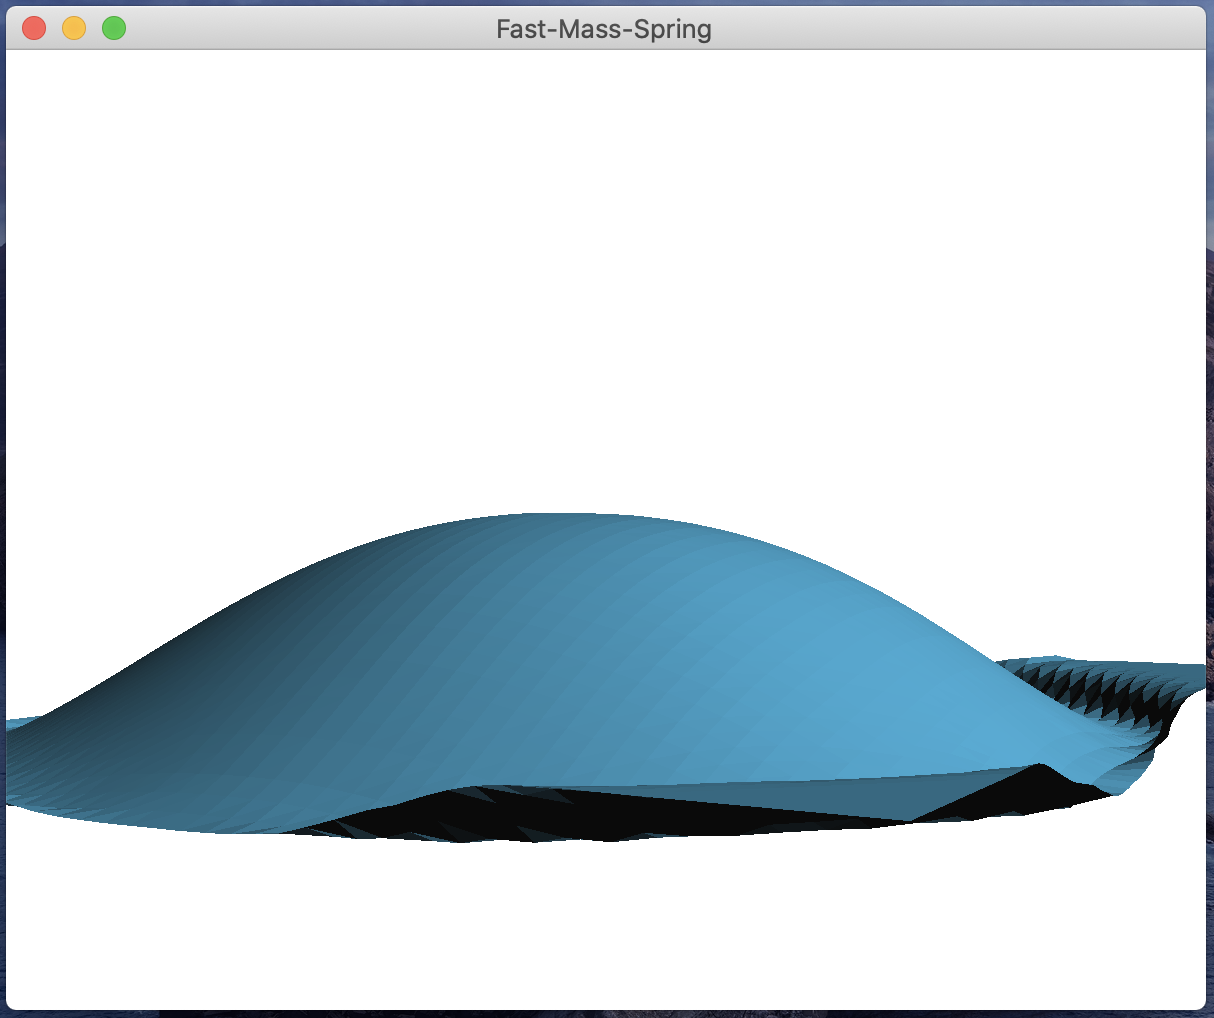
\includegraphics[scale=0.25]{./circle2.png}
	\caption{Demo of cloth simulation}
\end{figure}
For the solver part, I used the method described in the paper ``Fast Simulation of 
Mass-Spring Systems, Tiantian Liu, 2013'' to achieve real-time efficiency with details 
better preserved animation.\\
The demo program is compiled under \texttt{macOS 10.15} with \texttt{Apple clang 12.0} 
with 3rd party libraries: \texttt{OpenGL, glm, Eigen3}, and it's tested that it can 
preform simple cloth animations correctly.

\section{Implementation Details}
\subsection{Mesh generation}
For a given cloth with regular shape, it's simple to implement a mesh generation algorithm.
For example, the mesh for a rectangular cloth can be generated as the following figure
\begin{figure}[H]
	\centering
	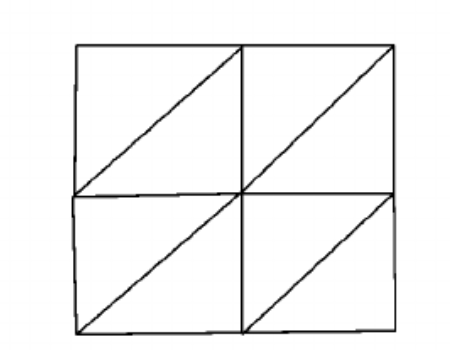
\includegraphics[scale=0.5]{./mesh.png}
	\caption{Mesh of rectangle}
\end{figure}
In this demo program, I just divide the rectangle into $m*n$ parts, and then divide each 
part into 2 triangles by its diagonal.\\
But for more complex shapes, we may need more complex algorithms like Delaunay triangulation
(it's not implemented in this assignment).\\

\subsection{Mass spring system construction}
For a simple rectangular cloth, the mass-spring system can be constructed as the following 
figure:
\begin{figure}[H]
	\centering
	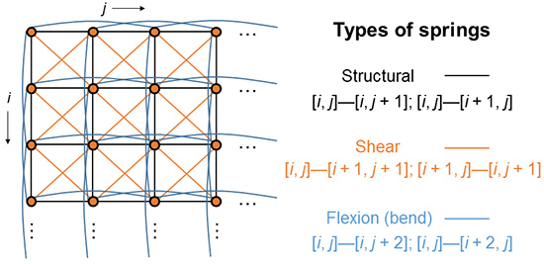
\includegraphics[scale=0.4]{./img2.png}
	\caption{Mass spring system}
\end{figure}
There are 3 types of springs:\\
\begin{enumerate}
	\item Structural springs: connect $M(i,j)$ with $M(i, j+1)$ and $M(i+1,j)$
	\item Shearing springs: connect $M(i,j)$ with $M(i+1, j+1)$, connect $M(i+1,j)$ with $M(i,j+1)$
	\item Bending springs:  connect $M(i,j)$ with $M(i, j+2)$ and $M(i+2,j)$
\end{enumerate}
When the masses is given, the springs can be simply constructed by the equation shown above.

\subsection{Mass spring solver}
Up to now, the mass spring system is already done, we just need to solve this system by the 
method described in the paper. The details and proof of these equations are shown in the paper, 
so I just introduce the equations used in my implementation.\\
First, we calculate the mass matrix $M \in \mathbb{R}^{3n\times 3n}$:
$$M(i, j) = diag(m_1, m_1, m_1, \ldots, m_i, m_i, m_i, \ldots, m_n, m_n, m_n)$$
Then, calculate the matrix $L\in \mathbb{R}^{3n\times 3n}$:
$$L = (\sum_{i=1}^{s}k_iA_iA_i^T)\otimes I_3$$
where $A_i \in \mathbb{R}^n$ is the incidence vector of i-th spring, and $I_3$ is the $3\times3$ 
identity matrix, and $s$ provides the number of springs. In this simple demo, the number of springs
$s = (n-1)(5n-2)$, which equals to the number of sum of 3 types of springs.\\
Then we need to build the matrix $J\in \mathbb{R}^{3n\times 3s}$: 
$$S = (\sum_{i=1}^{s}k_iA_iS_i^T)\otimes I_3$$
Here, $S_i$ denotes i-th spring indicator, where $S_{i,j} = \delta(i, j)$, and we denote the 
external force as $f_{ext} \in \mathbb{R}^{3n}$. Then we can minimize the energy:
$$E = \min_{d \in U}\frac{1}{2}x^TLx - x^TJd + x^T f_{ext}$$
We aggregate the external force and inertia into a vector $b$ and we can rewrite this 
optimtzation problem as:
$$\min_{x\in\mathbb{R^{3m}}, d \in U}\frac{1}{2}x^T(M+h^2L)x - h^2x^TJd + x^T b$$
Starting with an initial guess for $x$, we can first perform a local step: 
fix $x$ and compute the optimal $d$. Second, we perform a global step: fix $d$ and 
compute the optimal $x$, repeating this process until a maximal number of iterations
reached.\\ 
And for the constraints (collision), note that any translation of $x$ can be accomplished 
by appropriately chosen $f_{ext}$. Therefore, we can short-circuit this process and instead of 
computing $f_ext$, we directly compute by collision response routines and move $x$ to the 
collision-free state, instead of calculating the collision forces explicitly.\\
Thanks to \texttt{Eigen} provides us a efficient and easy to use API for matrix computation 
and optimiazation, the solver program can be done within 200 lines of code.\\

\section{Results}
In this assignment, I perform 2 different animation in the demo. The first one is 
a square cloth dropped and collided with a fixed square, and the second one is a square
cloth getting a impulse (an straight up external force) on a circle area at its center 
while dropping.\\
(1) Results of the first demo:
\begin{figure}[H]
	\centering
	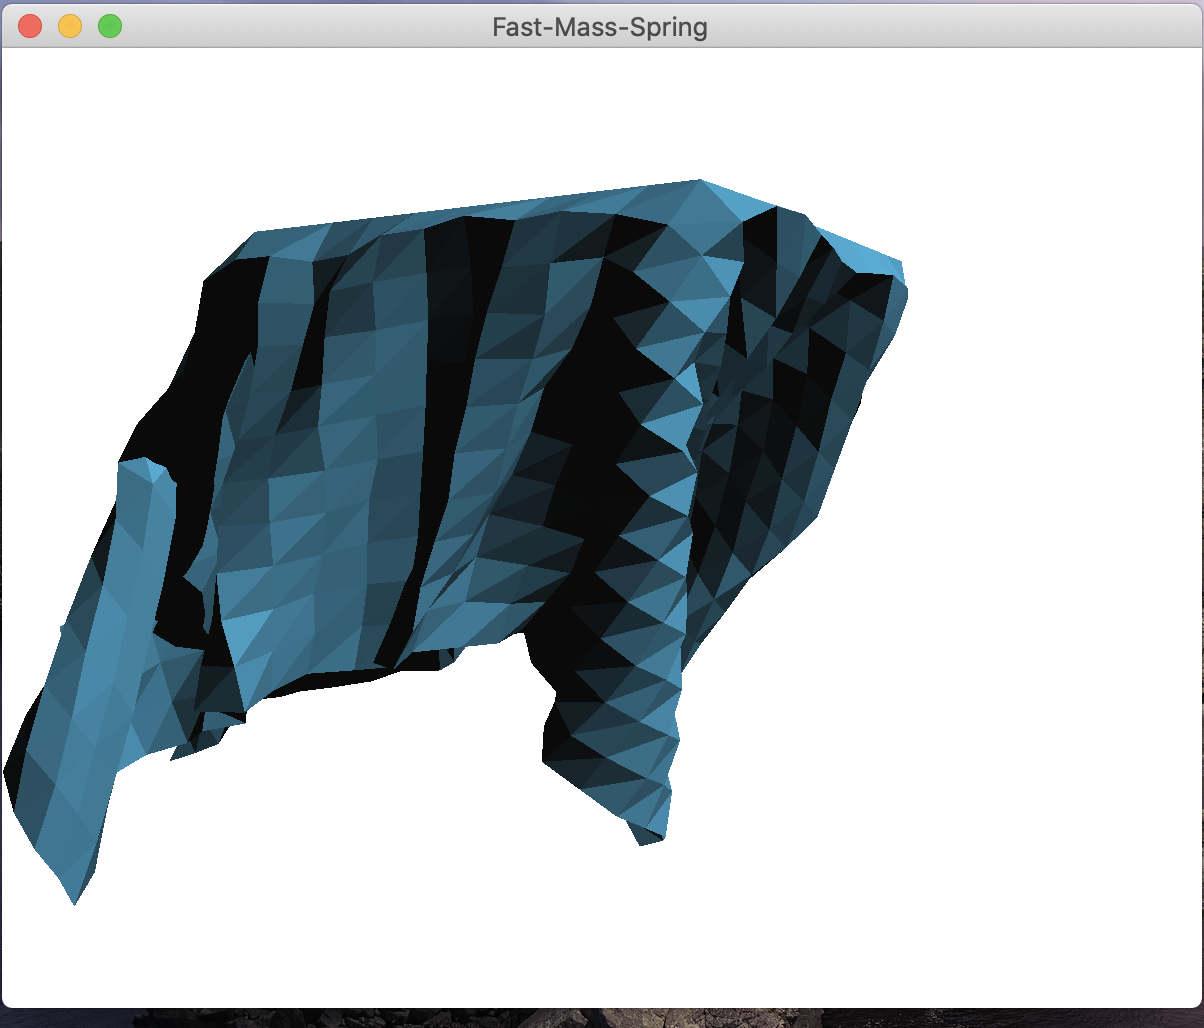
\includegraphics[scale=0.2]{./square1.png}
	\caption{collision between cloth and a fixed square - 1}
\end{figure}

\begin{figure}[H]
	\centering
	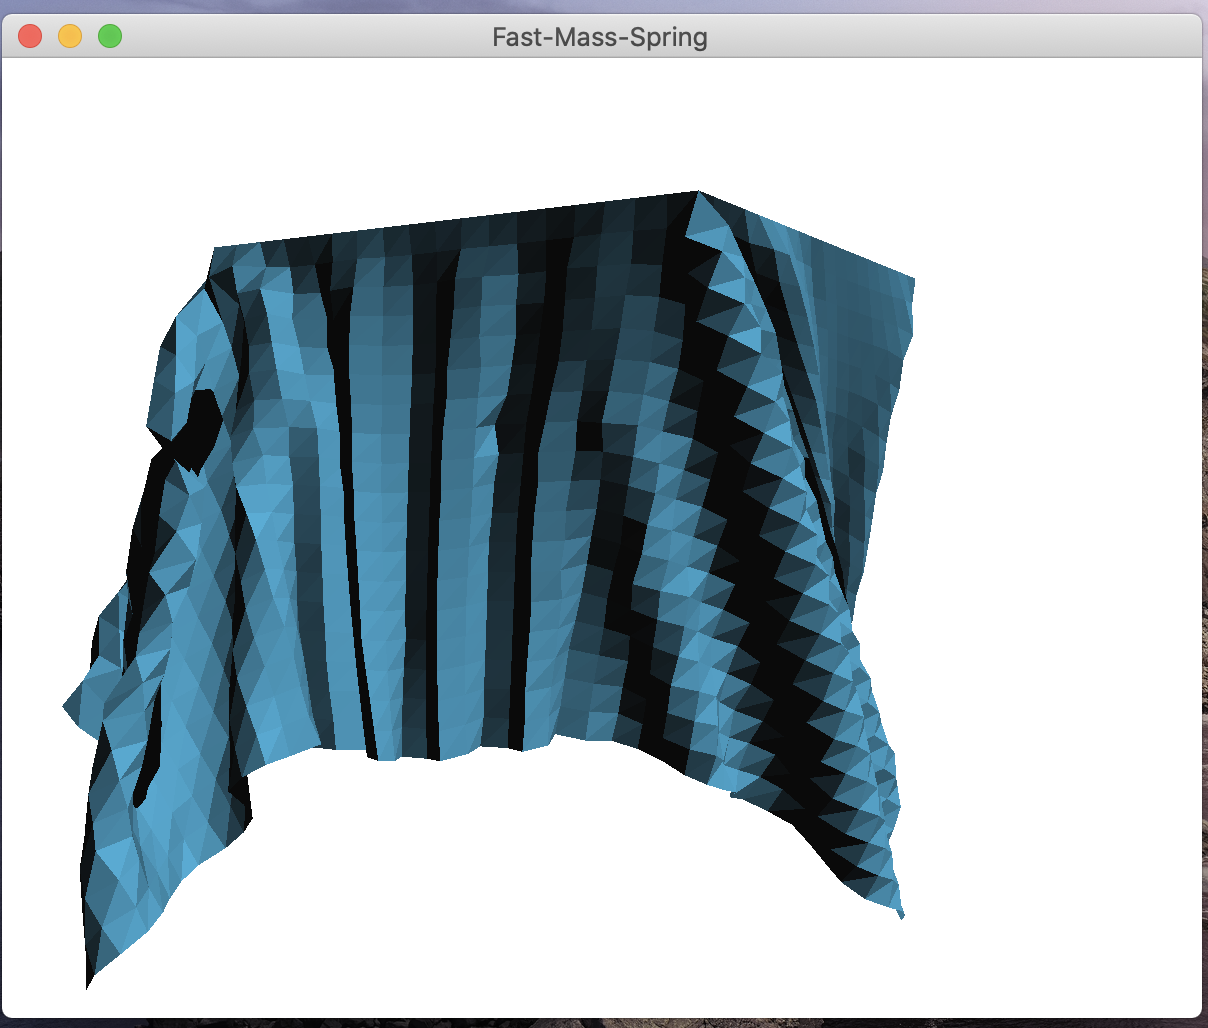
\includegraphics[scale=0.2]{./square2.png}
	\caption{collision between cloth and a fixed square - 2}
\end{figure}

(2) Results of the second demo:
\begin{figure}[H]
	\centering
	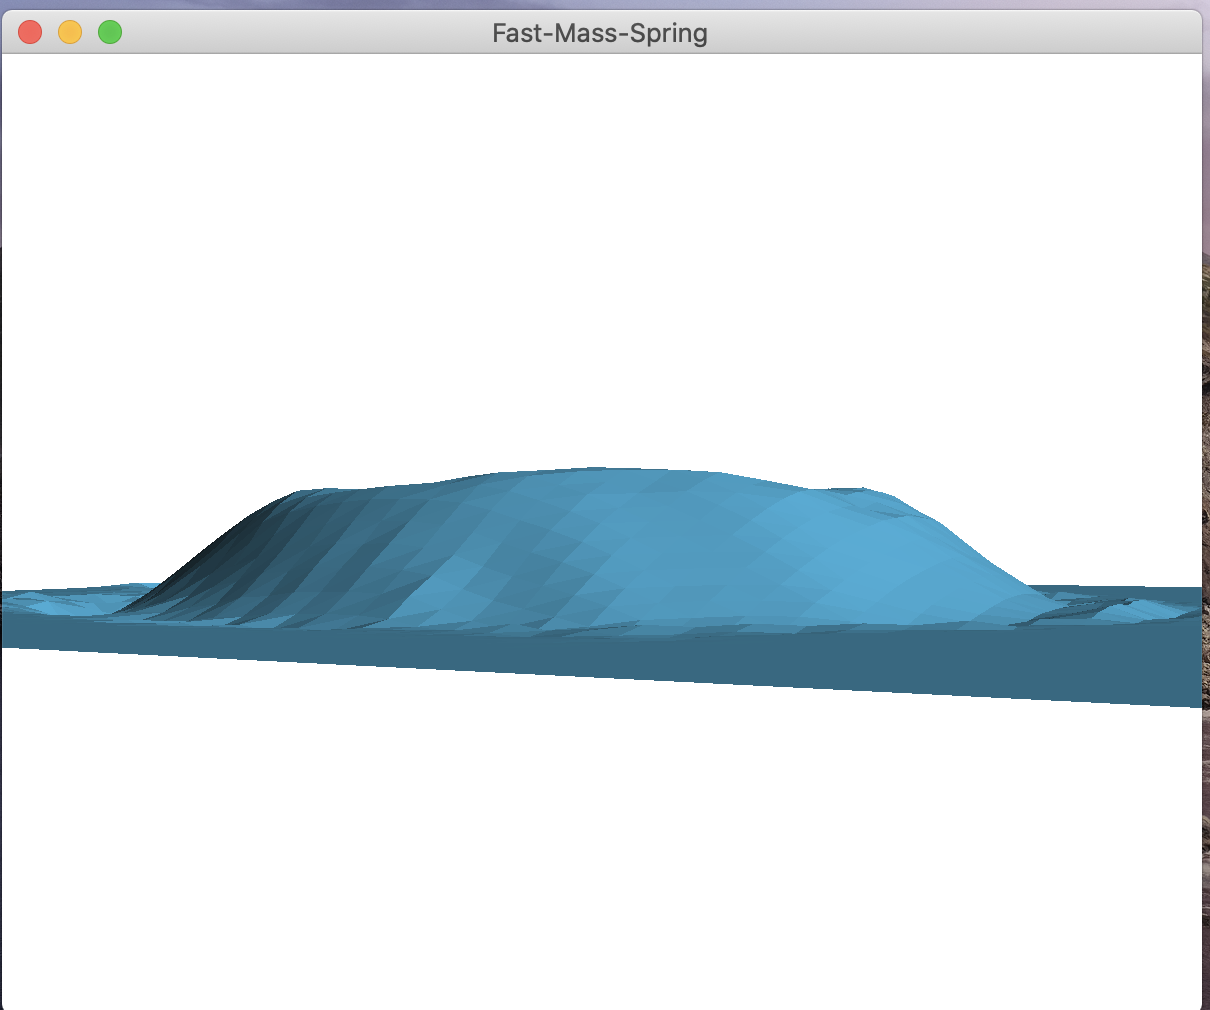
\includegraphics[scale=0.2]{./circle1.png}
	\caption{Circle impulse on the cloth - 1}
\end{figure}

\begin{figure}[H]
	\centering
	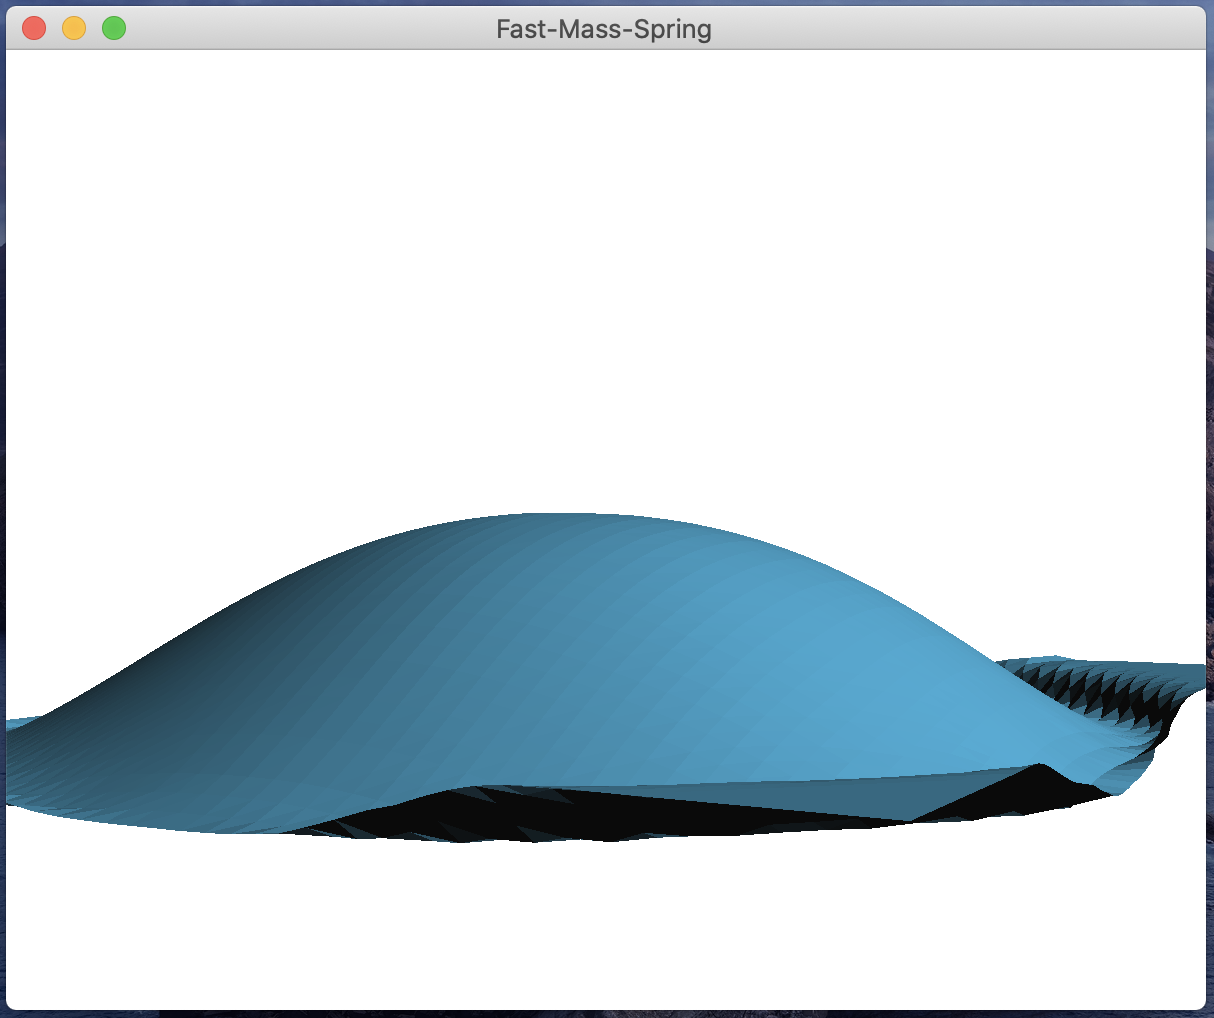
\includegraphics[scale=0.2]{./circle2.png}
	\caption{Circle impulse on the cloth - 2}
\end{figure}


\end{document}
